\setchapterpreamble[u]{\margintoc}
\chapter{Transport Level Security}
\labch{chapter5}

Protocolli analizzati: 
\begin{itemize}
    \item TLS (standard che deriva da SSL - Socket Security Level);
	\item HTTPS e SSH, che si appoggiano a TLS.
\end{itemize}

TLS/SSL sono state create per proteggere i Web Server e rendere sicura la comunicazione col client, a causa di una serie di caratteristiche intrinseche del web:
\begin{itemize}
    \item I web server sono relativamente semplici da configurare e gestire;
	\item Il contenuto è sempre più semplice da sviluppare;
	\item L'architettura sottostante è molto complessa, e può nascondere molti buchi di sicurezza;
	\item Un web server exploitato potrebbe essere usato per attaccare la rete dell'azienda che lo possiede;
	\item Gli utenti casual e non addestrati nella sicurezza sono i clienti comuni dei servizi basati su web server.
\end{itemize}
Gli utenti devono essere protetti sa server web malevoli e viceversa.

Le minacce sul web possono violare l'integrità, la confidenzialità, la disponibilità (DDoS) e l'autenticità.

La posizione dei protocolli di sicurezza rispetto allo stack del protocollo TCP/IP è mostrata in figura \ref{fig:5-1}.

\begin{figure}
    \centering
    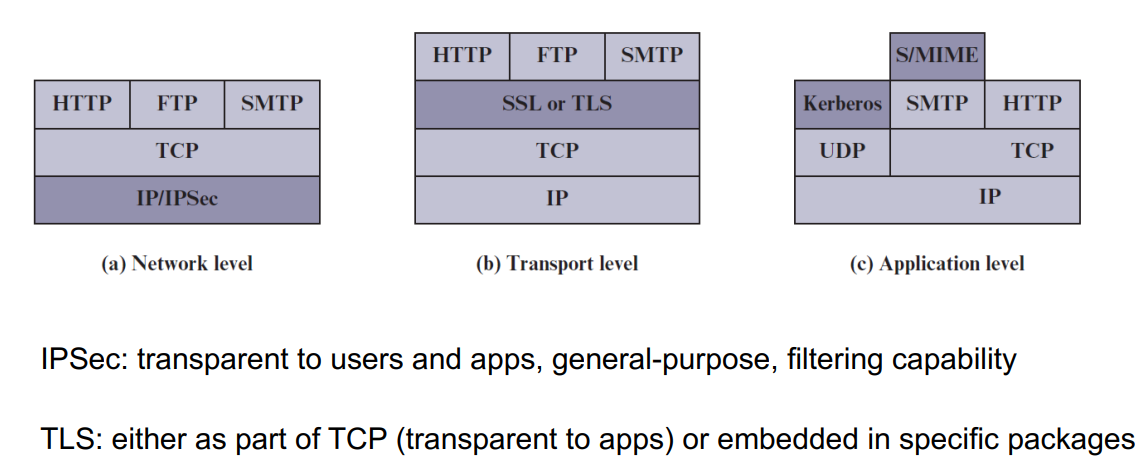
\includegraphics[width=1\textwidth]{images/chapter5/5-1.png}
    \caption{Scambio dei messaggi.}
    \label{fig:5-1}
\end{figure}

\section{Transport Level Security}
\begin{itemize}
    \item Si compone di una suite di protocolli usati in una sequenza ben precisa;
	\item È uno dei servizi di sicurezza più usati;
	\item Evolve da SSL;
	\item Si appoggia a TCP;
	\item Può venire fornito come parte del protocollo sottostante (TCP) oppure incorporato all'interno di specifici pacchetti;
	\item La maggior parte dei browser e web server lo implementano.
\end{itemize}

TLS si compone di una suit di protocolli:
\begin{itemize}
    \item Protocolli per stabilire la comunicazione e gli scambi di dati necessari ad avviare il protocollo:
	\begin{itemize}
	    \item Handshake protocol, per aprire la comunicazione tra due entità che non si conoscono  e decidere come scambiarsi le prime info necessarie alla prosecuzione del protocollo;
		\item Change chiper spec protocol, per cambiare l'algoritmo crittografico stabilito durante l'handshake;
		\item Alert protoco, per notificare situazione di warning;
		\item HTTP;
		\item Heartbeat protocol.
	\item Record protocol, che rende sicuri i dati dell'applicazione.
	\end{itemize}
\end{itemize}

L'architettura di TLS ha 2 componenti principali:
\begin{itemize}
    \item Connessione TLS: in generale una connessione è un "trasporto" che fornisce un servizio adatto al contesto in cui è stabilita. In TLS le connessioni sono relazioni peer-to-peer. Sono transienti e associate ad una sola sessione.
	\item Sessione TLS: si tratta di un'associazione tra un client e un server ed è creata tramite il protocollo di handshake. Definisce una serie di parametri crittografici per la sicurezza (lunghezza chiavi, protocollo crittografico da usare, …) condivisi tra tutte le connessioni associate alla sessione (evito di negoziare i parametri per ogni connessione).
\end{itemize}

I parametri scambiati in una sessione sono:
\begin{itemize}
    \item Identificatore della sessione;
	\item Certificato dei peer, nella versione X509.v3. Può essere nullo, in quanto il client potrebbe esserne sprovvisto;
	\item Algoritmo di compressione dei dati;
	\item Specifiche per la cifratura, come l'algoritmo di crittografia, l'algoritmo di hash per il calcolo del MAC, e altri attributi necessari alla crittografia;
	\item Master Secret, un segreto di 48 byte condiviso tra client e server;
	\item Una flag per specificare se la sessione può essere usata per aprire una nuova connessione.
\end{itemize}

I parametri di una connessione sono:
\begin{itemize}
    \item Server e client random, ovvero delle sequenze di byte scelte da client e server per ogni connessione;
	\item Server Write MAC Secret, ovvero al chiave segreta usata dal server nelle operazioni MAC sui dati inviati dal server;
	\item Client Write MAC Secret, ovvero al chiave segreta usata dal client nelle operazioni MAC sui dati inviati dal client;
	\item Server Write Key, ovvero la chiave segreta per la cifratura dei dati inviati dal server e decifrati dal client;
	\item Client Write Key, ovvero la chiave segreta per la cifratura dei dati inviati dal client e decifrati dal server;
	\item Initialization vector -> i pacchetti spediti con TLS seguono un meccanismo di block chain (la codifica di un pacchetto si basa sulla codifica del pacchetto precedente). Questo meccanismo necessita di un punto di partenza, per evitare che il primo pacchetto venga passato in chiaro, ovvero dell'initialization vector;
	\item Sequence numbers -> client e server usano delle sequenza di numeri, separate per pacchetti inviati e ricevuti, per evitare il riordino dei pacchetti da parte di un attaccante.
\end{itemize}

Obiettivi del Record Protocol:
\begin{itemize}
    \item Confidenzialità del messaggio;
	\item Integrità del messaggio.
\end{itemize}

Operazioni eseguite dal record protocol sul pacchetto:
\begin{itemize}
    \item Suddivide il pacchetto in frammenti;
	\item Comprime, senza perdere info, ciascun frammento;
	\item Calcola, per ciascun frammento compresso, il MAC e lo accoda -> integrità;
	\item Codifica il nuovo frammento -> confidenzialità;
	\item Antepone al frammento un header TLS.
\end{itemize}

\subsection{Passi dell'handshake protocol}

Nel corso di un handshake TLS, il client e il server operano insieme come segue:
\begin{itemize}
    \item Specificano la versione di TLS (TLS 1.0, 1.2, 1.3, ecc.) che utilizzeranno;
	\item Decidono quali suite di crittografia (vedi sotto) utilizzeranno;
	\item Autenticano l'identità del server tramite la chiave pubblica del server e la firma digitale dell'autorità di certificazione SSL;
	\item Generano chiavi di sessione per utilizzare la crittografia simmetrica dopo il completamento dell'handshake.
\end{itemize}

I passaggi all'interno di un handshake TLS sono (con  Diffie-Hellman autenticato):
\begin{enumerate}
    \item \textbf{'Client\_hello' e 'sever\_hello}: il client inizia l'handshake inviando un messaggio "hello" al server. Il messaggio includerà la versione TLS supportata dal client, le suite di crittografia supportate, una stringa di byte casuali che funziona come nonce e un id di sessione.
	In risposta al messaggio di saluto del client, il server invia un messaggio contenente il certificato SSL del server, la suite di cifratura scelta dal server e un suo nonce. Tipicamente è il server adatta le sue versioni di TLS e cypher suite a quelle del client o in generale ci si adatta a quello che richiede le versioni minori (Attenzione: un server/client che richiede versioni vecchie del protocollo potrebbe essere rischioso/malevolo);
	\item \textbf{Certificato e pre\_master\_secret del server}: il server invia il proprio certificato e il sua pre\_master\_secret che ha generato. Richiede, opzionalmente, al client il suo certificato;
	\item \textbf{Autenticazione e scambio chiavi}: il client verifica il certificato del server con l'autorità di certificazione che lo ha emesso. Ciò conferma che il server è chi dice di essere e che il client sta interagendo con l'effettivo proprietario del dominio. Se richiesto e se in possesso, il client può inviare il proprio certificato al server. Il client invia il proprio pre\_master\_secret;
	I due pre\_masetr\_secret vengono usati per generare il master\_secret, che sta alla base di tutte le chiavi usate durante la sessione;
	\item \textbf{Termine dell'handshake}: client e server raccolgono l'insieme di messaggi che si sono scambianti fin'ora, ne fanno l'hash (cifrato con una chiave generata a partire dal master\_secret) e verificano che i due valori ottenuti corrispondano. Questo permette di verificare che nessun attore si sia messo in mezzo allo scambio.
\end{enumerate}

 \begin{figure}
    \centering
    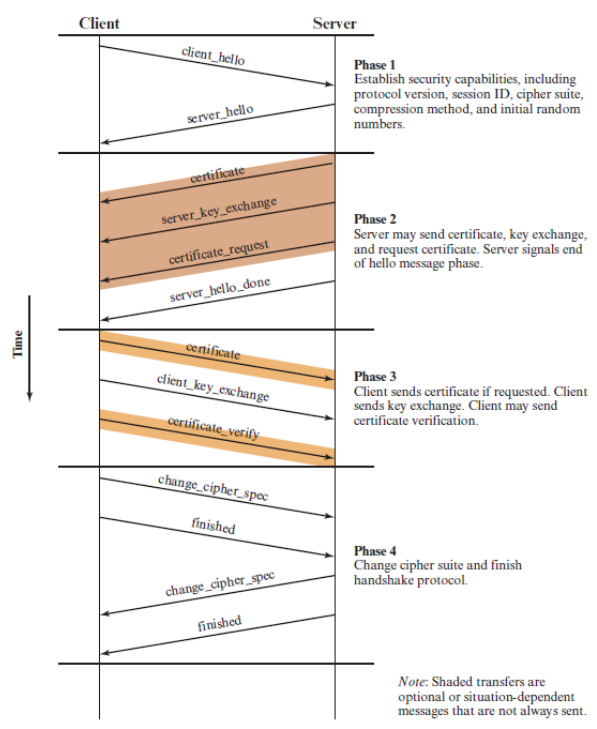
\includegraphics[width=1\textwidth]{images/chapter5/5-2.png}
    \caption{Passi dell'hasdshake protocol.}
    \label{fig:5-2}
\end{figure}

Fino all'ultima versione di SSL, il pre\_master\_secret era generato solo dal client e la crittografia usata per cifrare era RSA: 
\begin{itemize}
    \item Il server fornisce il suo certificato al client;
	\item Il client preleva la chiave pubblica del server dal certificato (dopo averlo verificato) e la usa per cifrare il pre\_master\_secret da lui generato; 
	\item Il server decifra il pre\_master\_secret ricevuto dal client  con la propria chiave privata;
	\item Entrambi i principals posseggono ora il pre\_master\_secret e possono generare il resto delle chiavi.
\end{itemize}
	
In TLS 1.3 l'suo di RSA (chiamato RSA statico) è stato deprecato, in quanto soffre di una debolezza importate: non rispetta la perfect forward secrecy. Supponiamo di aver stabilito una sessione con successo e di aver terminato l'handshake il 1° Luglio. Inizio quindi a creare delle connessioni, ognuna con la propria chiave generata a partire dalla master\_key, che durano per diverso tempo.  Il 30 di Luglio la chiave privata del server viene compromessa. Lo stesso giorno la craccatura viene scoperto e il certificato revocato. Da ora in poi infatti tutte le comunicazioni potrebbero essere compromesse. Anche le comunicazioni passate (1 - 30 Luglio) sono compromesse, in quanto l'attaccante, se ha registrato i messaggi scambiati durante l'handshake protocol, può decifrare quello contenente il pre\_master\_secret, creare il master\_secret (il metodo su come crearlo è deciso durante l'handshake) e in cascata tutte le altre chiavi. Può ora decodificare, sempre supponendo che li abbia registrati, tutti i messaggi scambiati nella sessione.

In TLS 1.3 si usa Diffie-Hellman autenticato. L'autenticazione può essere raggiunta, ad esempio, se client e server possiedono entrambi un certificato. IN questo caso ciascuno può cifrare la mezza chiave con la chiave pubblica dell'altro. A seconda del tipo di servizi/info forniti dal server, ci si può accontentare anche solo del certificato di quest'ultimo.

Nelle versioni precedente alla 1.3 di TLS,  Diffie-Hellman è comunque usabile (previo accordo tra le parti), ma non obbligatorio.

Dal master\_secret viene derivata:
\begin{itemize}
    \item Server Write MAC key;
	\item Client Write MAC key;
	\item Server Write Key;
	\item Client Write Key;
	\item Initialization vector di client e server.
\end{itemize}

Gli attacchi a TLS possono essere raggruppati in:
\begin{itemize}
    \item Attacchi all'handshake protocol;
	\item Attacchi al record protocol o ai protocolli usati dai dati dell'applicazione;
	\item Attacchi alla public key infrastructure;
    \item Altri tipi di attacchi.
\end{itemize}

\section{Secure Shell (SSH)}

Protocollo per comunicazioni di rete sicure progettato per essere relativamente semplice e poco costoso da implementare. La versione iniziale, SSH1, era focalizzata sul fornire un login da remoto sicuro su altre macchine per sostituire TELNET e altri schemi di accesso remoto che non fornivano sicurezza. 
Fornisce ora anche una capacità client/server più generale e può essere utilizzato per funzioni di rete come il trasferimento di file e la posta elettronica.
SSH2 corregge una serie di falle di sicurezza nello schema originale.

Le applicazioni client e server SSH sono ampiamente disponibili per la maggior parte dei sistemi operativi come mezzo per:
\begin{itemize}
    \item Accesso da remoto;
	\item X tunneling.
\end{itemize}

\subsection{Stack del protocollo}
Il protocollo si compone di due layer (figura \ref{fig:5-3}):
\begin{itemize}
    \item Transport Layer Protocol: fornisce l'autenticazione del server, la riservatezza dei dati, e l'integrità dei dati con forward secrecy (ad esempio, se una chiave viene compromessa durante una sessione, la sua conoscenza non minaccia la sicurezza delle sessioni precedenti). Lo strato di trasporto può opzionalmente fornire compressione;
	\item User Authentication Protocol: autentica gli utenti al server;
    \item Connection protocol.
\end{itemize}

\begin{figure}
    \centering
    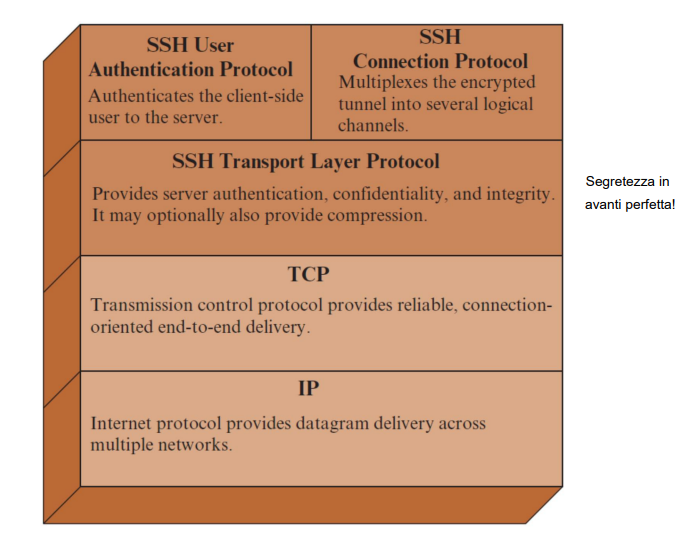
\includegraphics[width=1\textwidth]{images/chapter5/5-3.png}
    \caption{Layer SSH.}
    \label{fig:5-3}
\end{figure}

\subsection{SSH Transport Layer Protocol}

Basi:
\begin{itemize}
    \item L'autenticazione del server avviene a livello di trasporto, basandosi sul possesso di una coppia di chiavi pubblica/privata da parte del server;
	\item Un server può avere più chiavi host che utilizzano diversi algoritmi di cifratura asimmetrica;
	\item Più host possono condividere la stessa chiave host;
	\item La chiave host del server viene utilizzata durante lo scambio di chiavi per autenticare l'identità dell'host;
	\item RFC 4251 impone due modelli di trust alternativi:
	\begin{itemize}
	    \item Il client dispone di un database locale che associa ogni nome host con la chiave host pubblica corrispondente;
		\item L'associazione host-key è certificata da una Certification Authority di fiducia. Il client conosce solo la chiave radice della CA e può verificare la validità di tutte le chiavi host certificate da essa.
	\end{itemize}
\end{itemize}

\begin{figure}
    \centering
    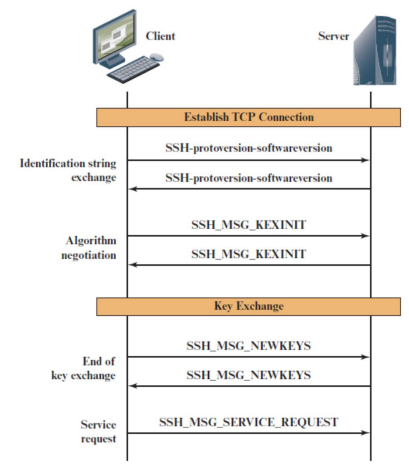
\includegraphics[width=0.9\textwidth]{images/chapter5/5-4.png}
    \caption{Scambio di messaggi in SSH Transport Layer Protocol.}
    \label{fig:5-4}
\end{figure}

Messaggi scambiati (figura \ref{fig:5-4}):
\begin{enumerate}
    \item Il client stabilisce una connessione TCP col server. Questo passo viene fatto con TCP e non con il Transport Layer Protocol;
	\item Identification string exchange: il client invia una stringa di identificazione. Il server risponde con una proprie stringa di identificazione;
	\item Algorithm negotiation: ogni parte invia una lista degli algoritmi supportati (per scambio chiavi, cifratura, MAC, compressione). Per ogni categoria, l'algoritmo scelto è il primo nella lista del client che il server supporta (il client ordina le entry della lista come vuole);
	\item Key exchange: lo scambio può avvenire con 2 versioni di Diffie-Hellman (DH). Lo scambio avviene come segue:
	\begin{enumerate}
	    \item Il client invia la sua mezza chiave di DH;
		\item Il server firma l'hash della mezza chiave, della chiave Ks e delle stringhe di identificazione con la chiave privata dell'host e invia al client la chiave pubblica dell'host Ks, l'altra mezza chiave di DH e l'hash firmato;
		\item Il client verifica la chiave pubblica dell'host KS con il suo database locale o con la CA.
	\end{enumerate}
	\item End of key exchange: si segnala la fine dello scambio con uno specifico pacchetto;
	\item Service request: il client invia un pacchetto nel quale richiede SSH User Authentication protocol o SSH Connection protocol.
\end{enumerate}

I pacchetti SSH scambiati hanno i seguenti campi:
\begin{enumerate}
    \item Lunghezza del pacchetto, escluso i campi MAC e lunghezza paccheto;
	\item Lunghezza del padding;
	\item Payload eventualmente compresso;
	\item Padding, la cui dimensione è decisa il base all'algoritmo di cifratura usato;
	\item MAC, calcolato tentendo conto di tutti i 4 campi precedenti non cifrati.
\end{enumerate}

I campi 1, 2, 3, 4 vengono cifrati con l'algoritmo scelto.

Le chiavi utilizzate per la crittografia e il MAC sono generate usando:
\begin{itemize}
    \item La chiave DH segreta condivisa K;
	\item Il valore hash usato nello scambio delle chiavi H=hash(..K..);
    \item L'identificatore di sessione, che è uguale a H a meno che non vi sia stato un successivo scambio di chiavi dopo lo scambio di chiavi iniziale.
\end{itemize}

\subsection{SSH User authentication protocol}

Il protocollo di autenticazione utente fornisce i mezzi con cui il client viene autenticato sul server. Il protocollo usa sempre tre formati di messaggi:
\begin{itemize}
    \item Messaggio del client:
	\begin{itemize}
	    \item SSH\_MSG\_USERAUTH\_REQUEST
		\item Nome utente = identità che il client dichiara
		\item Service name = struttura a cui il client sta richiedendo l'accesso (generalmente SSH Connection Protocol)
		\item Method name = metodo di autenticazione utilizzato nella richiesta
	\end{itemize}
	\item Risposta negativa del server:
	\begin{itemize}
	    \item SSH\_MSG\_USERAUTH\_FAILURE
		\item Lista di metodi che potrebbero continuare il dialogo
		\item Booleano che indica il parziale successo
	\end{itemize}
	\item Risposta positiva del server:
	\begin{itemize}
	    \item SSH\_MSG\_ USERAUTH\_SUCCESS
	\end{itemize}
\end{itemize}

\begin{figure}
    \centering
    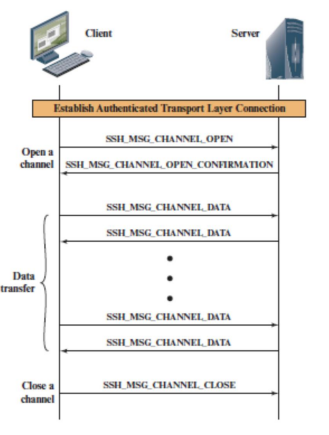
\includegraphics[width=0.9\textwidth]{images/chapter5/5-5.png}
    \caption{Scambio di messaggi per SSH User authentication protocol.}
    \label{fig:5-5}
\end{figure}

Scambio dei messaggi (figura \ref{fig:5-5}):
\begin{enumerate}
    \item Il cliente invia a SSH\_MSG\_USERAUTH\_REQUEST senza specificare il method name;
	\item Il server verifica se il nome utente è valido. In caso contrario, il server restituisce SSH\_MSG\_USERAUTH\_FAILURE con il valore di successo parziale false. Se il nome utente è valido, il server procede al passaggio 3;
	\item Il server restituisce SSH\_MSG\_USERAUTH\_FAILURE con un elenco di uno o più metodi di autenticazione da utilizzare;
	\item Il client seleziona uno dei metodi di autenticazione e invia un SSH\_MSG\_USERAUTH\_REQUEST con il nome del metodo e i campi specifici del metodo richiesti. A questo punto, potrebbe esserci una sequenza di scambi per eseguire il metodo;
	\item Se l'autenticazione ha esito positivo e sono necessari più metodi di autenticazione, il server procede al passaggio 3, utilizzando il valore di successo parziale true. Se l'autenticazione non riesce, il server procede al passaggio 3, utilizzando il valore di successo parziale false;
	\item Quando tutti i metodi di autenticazione richiesti hanno esito positivo, il server invia un messaggio SSH\_MSG\_USERAUTH\_SUCCESS e il protocollo di autenticazione è terminato.
\end{enumerate}

Metodi di autenticazione:
\begin{itemize}
    \item Chiave pubblica: 
	\begin{itemize}
	    \item Il client invia un messaggio al server che contiene la chiave pubblica del client, con il messaggio firmato con la chiave privata del client;
		\item Quando il server riceve il messaggio, verifica se la chiave fornita è accettabile per l'autenticazione e, in caso affermativo, verifica se la firma è corretta.
	\end{itemize}
	\item Password: 
	\begin{itemize}
	    \item Il client invia un messaggio contenente una password in chiaro, cifrata dal Transport Layer Protocol (TLS);
	\end{itemize}
	\item Attraverso l'hosh:
	\begin{itemize}
	    \item L'autenticazione viene eseguita sull'host del client anziché sul client stesso;
		\item Questo metodo funziona facendo in modo che il client invii una firma creata con la chiave privata dell'host;
		\item Anziché verificare direttamente l'identità dell'utente, il server SSH verifica l'identità dell'host (perdo l'accountability in quanto non so chi è effettivamente connesso all'host).
	\end{itemize}
\end{itemize}

\subsection{SSH Connection Protocol}

Il protocollo di connessione SSH viene eseguito sopra l'SSH Transport Layer Protocol e presuppone che sia attiva una connessione autenticata sicura. La connessione di autenticazione sicura, denominata tunnel, viene utilizzata dal protocollo di connessione per multiplexare un numero di canali logici.

Canale:
\begin{itemize}
    \item Tutti i tipi di comunicazione tramite SSH sono supportati utilizzando canali separati;
	\item Entrambe le parti possono aprire un canale;
	\item Ad ogni canale, ogni lato associa un numero di canale univoco;
	\item Il flusso dei canali è controllato mediante un meccanismo a finestra;
	\item Nessun dato può essere inviato a un canale finché non viene ricevuto un messaggio che indica che lo spazio della finestra è disponibile;
	\item La vita di un canale procede attraverso tre fasi: apertura del canale, trasferimento dati, chiusura del canale.
\end{itemize}

Messaggi scambiati:
\begin{enumerate}
    \item \textbf{Apertura del nuovo canale}: la parte che desidera aprire il canale allora un numero locale per il canale e invia un messaggio di apertura, che contiene:
	\begin{itemize}
	    \item SSH\_MSG\_CHANNEL\_OPEN
		\item Tipo del canale, che identifica l'applicazione per il canale
		\item Il numero locale del canale
		\item Dimensione iniziale della finestra
		\item Dimensione massima dei pacchetti
		\item Info sui dati
	\end{itemize}
	2. Se l'altra parte è in grado di aprire il canale, invia un messaggio di conferma che contiene:
	\begin{itemize}
	    \item SSH\_MSG\_CHANNEL\_OPEN\_CONFIRMATION
		\item Il numero locale ricevuto
		\item Il numero locale allocato
		\item Dimensione della finestra e dei pacchetti per il traffico in entrata
	\end{itemize}
	In caso di insuccesso nell'apertura, il messaggio contiene:
	\begin{itemize}
	    \item SSH\_MSG\_CHANNEL\_OPEN\_FAILURE
		\item Codice che rappresenta il motivo del fallimento
	\end{itemize}
	\item \textbf{Data transfer}: scambio di dati tra le due parti;
	\item \textbf{Chiusura canale}: la parte che desidera chiudere il canale invia un messaggio a riguardo.
\end{enumerate}

Tipi di canale:
\begin{itemize}
    \item Sessione: esecuzione remota di un programma. Il programma può essere una shell, un'applicazione come il trasferimento di file o e-mail, un comando di sistema o un sottosistema integrato. Una volta aperto un canale di sessione, le richieste successive vengono utilizzate per avviare il programma remoto;
	\item X11: Si riferisce a X Window System, un sistema software per computer e un protocollo di rete che fornisce un'interfaccia utente grafica (GUI) per i computer in rete. X consente alle applicazioni di essere eseguite su un server di rete ma di essere visualizzate su una macchina desktop;
	\item Forwarded-tcpip: forwarding remoto della porta;
	\item Direct-tcpip: forwarding della porta locale.
\end{itemize}

Port forwarding (inoltro della porta):
\begin{itemize}
    \item Una delle funzionalità più utili di SSH;
	\item Offre la possibilità di convertire qualsiasi connessione TCP non sicura in una connessione SSH sicura (denominato anche tunneling SSH);
	\item Il traffico TCP in entrata viene consegnato all'appropriata applicazione in base al numero di porta (una porta è un identificatore di un utente di TCP);
	\item Un'applicazione può utilizzare più numeri di porta.
\end{itemize}

Supponiamo di avere un'applicazione client identificata dal numero di porta x e un'applicazione server identificata dal numero di porta y. Ad un certo punto, l'applicazione client richiama l'entità TCP locale e richiede una connessione al server remoto sulla porta y. L'entità TCP locale negozia una connessione TCP con l'entità TCP remota, in modo tale che la connessione colleghi la porta locale x alla porta remota y.

Per proteggere questa connessione, SSH è configurato in modo che SSH Transport Layer Protocol stabilisca una connessione TCP tra le entità client e server SSH, rispettivamente con i numeri di porta TCP a e b. Un tunnel SSH sicuro viene stabilito su questa connessione TCP. Il traffico dal client alla porta x viene reindirizzato all'entità SSH locale e viaggia attraverso il tunnel in cui l'entità SSH remota consegna i dati all'applicazione server sulla porta y. Il traffico nella direzione opposta viene reindirizzato in modo simile.

\begin{figure}
    \centering
    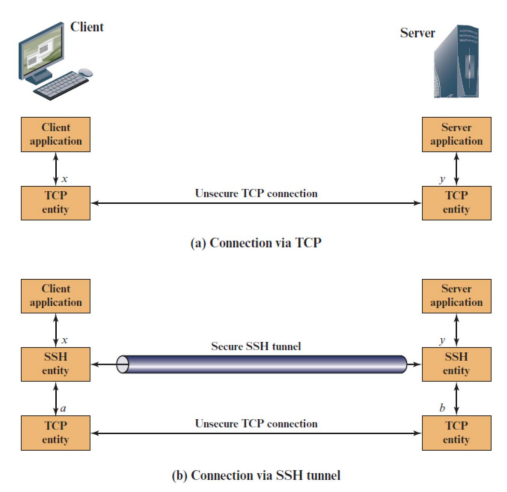
\includegraphics[width=1\textwidth]{images/chapter5/5-6.png}
    \caption{Scambio di messaggi per SSH User authentication protocol.}
    \label{fig:5-6}
\end{figure}

\section{Appunti aggiuntivi}

\subsection{Rollback attack in SSL}

La versione originale di SSL 3.0 prevedeva, nella fase iniziale dell'handshake, l'invio in chiaro da parte del client della versione di SSL supportata, insieme alle altre info di configurazione. Se il messaggio veniva catturato prima di arrivare al server, l'attaccante poteva facilmente modificare impostazioni come la versione, essendo non cifrata, inserendo ad esempio la versione 2.0, che non supporta il controllo con hash finale dello scambio di messaggi.
Per risolvere, SSL 3.0 ha deciso che il client, nel successivo messaggio che contiene la mezza chiave, vada ad inserire anche la versione di SSL che lui sta utilizzando. Ovviamente questo messaggio è cifrato con la chiave pubblica del server, e quindi sicuro.

\subsection{Combinare HTTPS con HTTP}

Tralasciando i casi di errori di programmazione dove uno script attiva erroneamente HTTP, esistono casi in cui i siti web accettano di servire sia HTTP che HTTPS (es: arrivo al sito con HTTP, vengo rediretto al login con HTTPS; cerco nel sito con HTTP, vado al checkout con HTTPS). In questi casi l'attaccante, se riesce a catturare il messaggio del client, può modificarne il contenuto sostituendo la richiesta del protocollo HTTPS con quello HTTP.

\subsection{Vulnerabilità nel salvataggio delle chiavi}

La chiave privata può essere protetta nel server in più modi:
\begin{itemize}
    \item  Usando uno specifico HW che genera coppie di chiavi SSL, mantiene la chiave privata e si occupa della cifratura. L'HW è costoso e richiede specifici driver nel server;
	\item Mantenendo la chiave sul server cifrata;
	\item Mantenendo la chiave sul server non cifrata (MOLTO comune).
\end{itemize}
 
\subsection{Vulnerabilità nella gestione dei certificati}

Se un nodo della catena è compromesso, tutto il sottoalbero è compromesso.


